\section{Definition des Begriffes}

\begin{frame}{Der Begriff \textit{tarnen}}
  Definition des Duden:
  \begin{block}{{\centering tar - nen}}
    jemanden, etwas vor dem Erkannt-, Gesehenwerden sch\"utzen,
    indem man es verh\"ullt oder der Umgebung angleicht
  \end{block}
\end{frame}

\section{Beispiele}
\begin{frame}{Ein Blick in die Natur.}
  \begin{figure}
    \centering
    \caption{Ein \textit{getarnter} Luchs im Dortmunder Zoo.}
    \includegraphics[width=0.6\textwidth]{images/luchs-do.JPG}
  \end{figure}
\end{frame}

\begin{frame}{Funktioniert das auch f\"ur Menschen?}
  \begin{figure}
    \centering
    \caption{Der Chinesische K\"unstler Liu Bolin tarnt sich. \cite{humanhide}}
    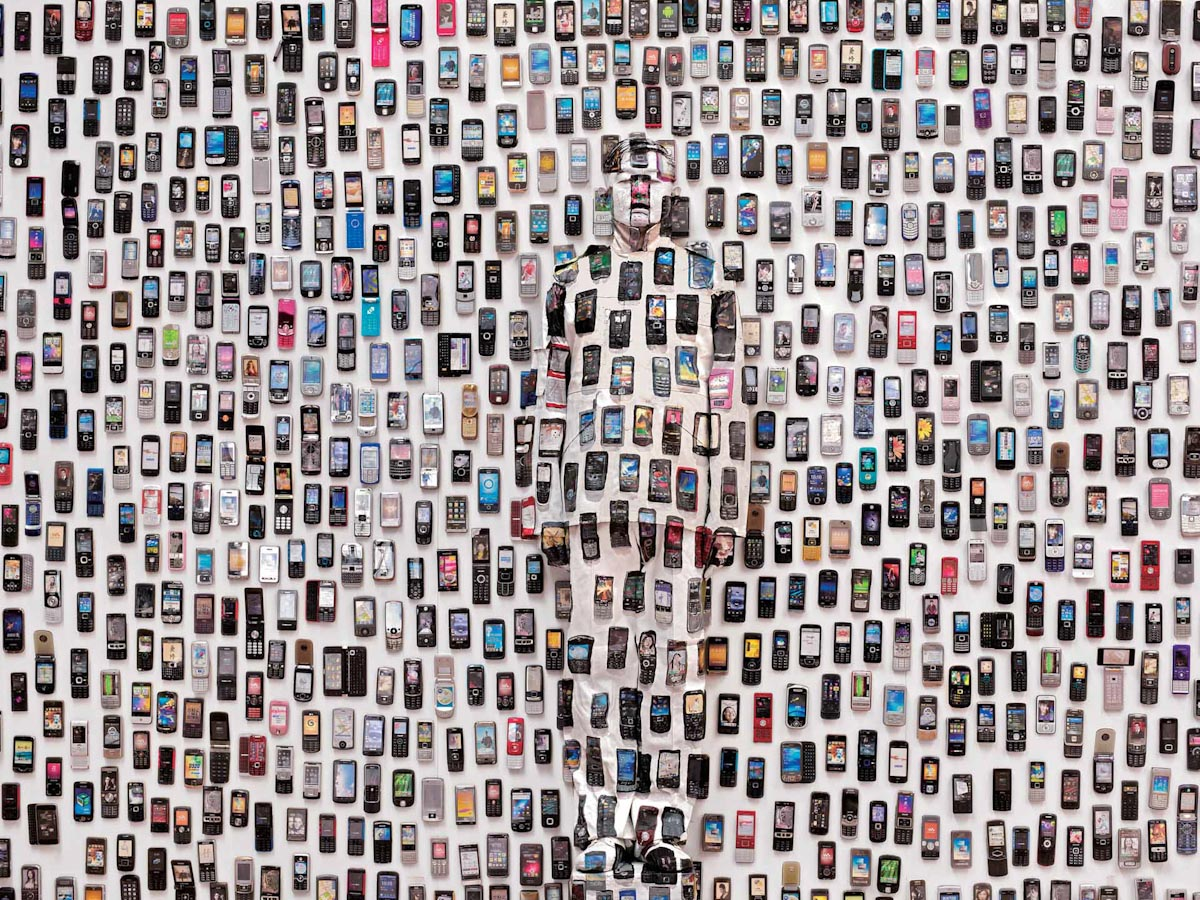
\includegraphics[height=0.8\textheight]{images/liubolin.jpg}
  \end{figure}
\end{frame}

\begin{frame}{Dynamisch statt statisch}
  Im Radarwellenbereich, $λ = \SI{10}{\centi\meter}$, können Flugzeuge getarnt werden.
  Der B-2 Spirit Tarnkappenbomer hat eine Radarreflexion eines kleinen Vogels.
  \begin{figure}
    \centering
    \begin{subfigure}{0.48\textwidth}
      \centering
      \caption{Eine Aufnahme der B-2 Spirit (US-Luftwaffe). \cite{b2spirit}}
      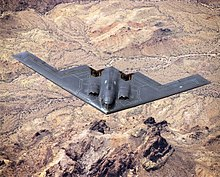
\includegraphics[width=0.7\textwidth]{images/b2spirit.jpg}
    \end{subfigure}
    \begin{subfigure}{0.48\textwidth}
      \centering
      \caption{Ein Bild eines Spatzen zum Vergleich. \cite{spatz}}
      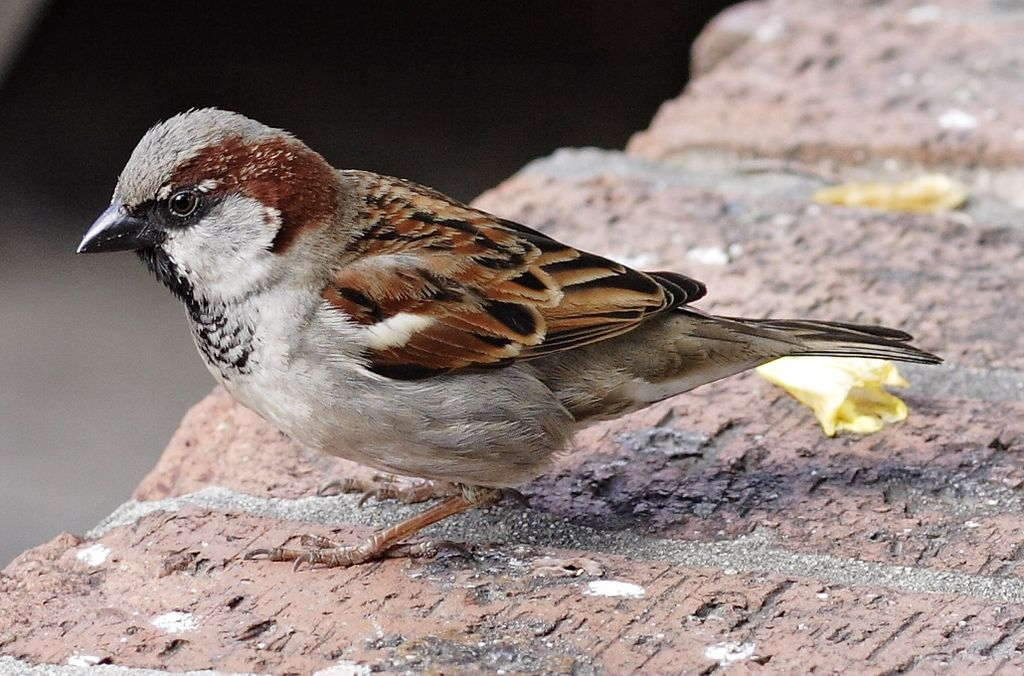
\includegraphics[width=0.7\textwidth]{images/spatz.jpg}
    \end{subfigure}
  \end{figure}
\end{frame}

\begin{frame}{Sichtbarer Bereich}
  \begin{columns}
    \begin{column}{0.48\textwidth}
      \begin{figure}
        \centering
        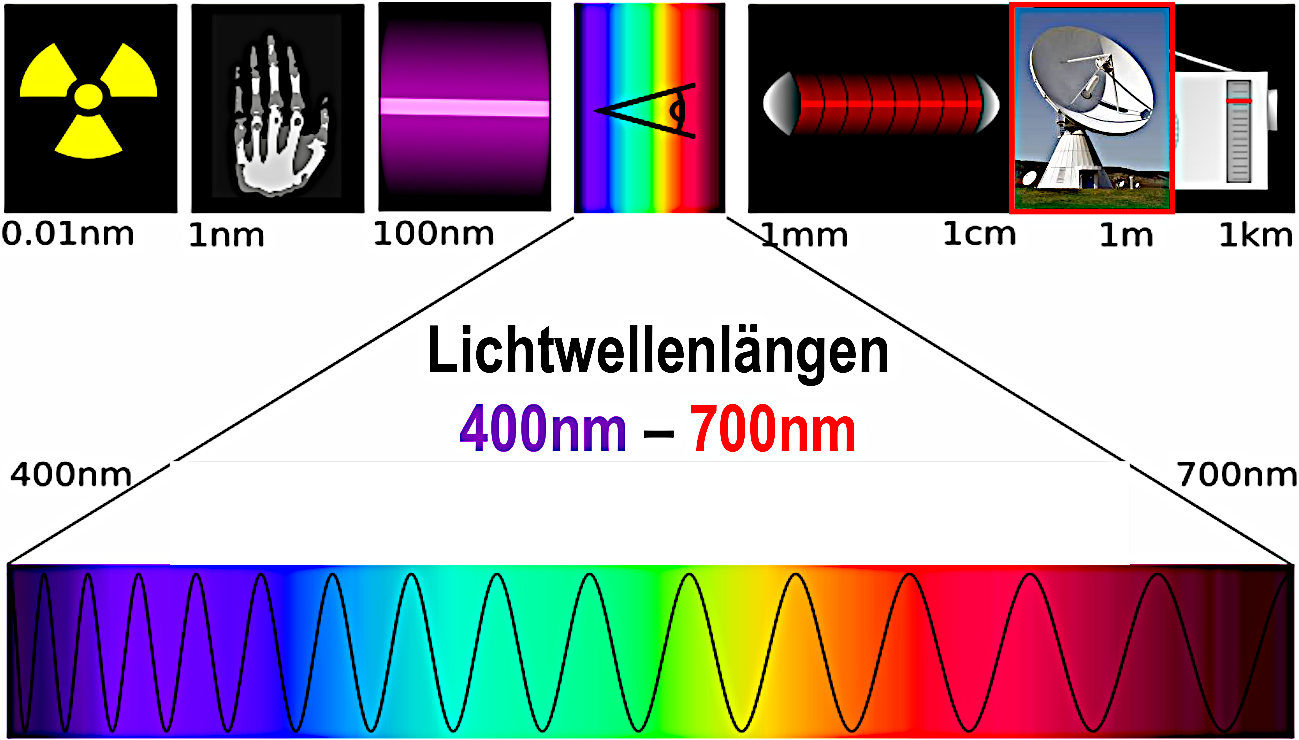
\includegraphics[width=\textwidth]{images/wellenbereich.png}
        \caption{Das Spektrum elektromagnetischer Wellen.}
      \end{figure}
    \end{column}
    \begin{column}{0.48\textwidth}
      Im optischen Bereich ist ein Objekt mit hoher Absorption leicht zu erkennen,
      da der Hintergrund nicht sichtbar ist. \\
      $\implies$ Das Licht muss um das Objekt herumgef\"uhrt werden.
    \end{column}
  \end{columns}
\end{frame}

\begin{frame}{Ablenkung von Licht}
  \begin{figure}
    \caption{Das schwarze Loch in Messier 87, \cite{m87}}
    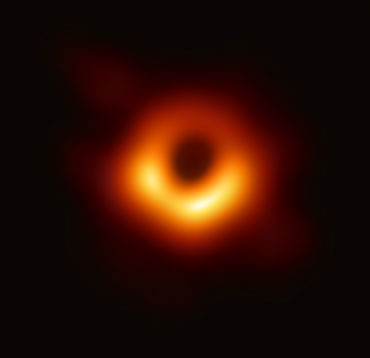
\includegraphics[height=0.8\textheight]{images/m87.jpg}
  \end{figure}
\end{frame}
